\documentclass[12pt]{article}
\oddsidemargin=0.0in
\evensidemargin=0.0in
\textwidth=6.5in
\topmargin=-0.55in
\textheight=9.3in
\usepackage{hyperref}
\usepackage{graphicx}
\usepackage{amsmath}

\begin{document}
\pagestyle{empty}
 
\begin{center}
{\LARGE {\bf Homework Six}}\\
\bigskip
{\Large {\bf Calculus I}}\\
\bigskip
{\Large {\bf College of the Atlantic}}\\
\bigskip
{ {\bf Due Friday, October 21, 2022}}\\ 
\end{center}
\medskip


\noindent There are two parts to this assignment.\\

\noindent {\bf Part 1: WeBWorK}.  Do Homework 06A and 06B on
WeBWorK.  The WeBWorK page is here: 
\url{https://webwork.runestone.academy/webwork2/coa-feldman-es1024i-fall-2022/}.
I recommend doing the WeBWorK part of the homework first.  This will
enable you to benefit WeBWorK's instant feedback before you do part
two.\\ 


\noindent {\bf Part 2: Non-WeBWorK problems}.  Here are some
instructions for how to submit this part of the assignment.
\begin{itemize}
  \setlength{\itemsep}{0mm}
\item Do the problems by hand using pencil (or pen) and paper.
  There is no need to type this assignment.
%\item If you like working on a tablet, go for it. 
\item Make a pdf scan of your work using genius scan or some
  similar scanning app.  Please make the homework into a single
  pdf, not multiple pdfs.
\item Submit the assignment on google classroom.  Please don't
  email it to me.
  %(Between my two classes I will be receiving
  %around 60 assignments a week.  Keeping track of them all in email 
  %is challenging.)
\item If you want, you can do the non-WeBWorK problems in pairs and
  submit only one assignment for the two of you. \\
\end{itemize}

\noindent Here are some non-WeBWorK problems.\\


\begin{enumerate}
\setlength{\itemsep}{33mm}

\item The temperature $T$ of an object as a function of time is
  described by the following function:
  \begin{equation}
    T(t) \, = \, 20 + 40e^{-kt} \;,
  \end{equation}
  where $k = 0.003$, $t$ is measured in seconds, and temperature is
  measured in Celsius.
  \begin{enumerate}
    \setlength{\itemsep}{8mm}
  \item Sketch $T(t)$.
  \item What is the initial temperature of the object?
  \item What is the temperature of the object after a long time (as
    $t$ gets very large)?
  \item At what time is the temperature $30$ Celsius?
  \item At $t=200$, at what rate is the object cooling?
  \end{enumerate}


  
\item Consider the function $f(x) = xe^x$.
  \begin{enumerate}
    \item For what values of $x$ is $f(x)$ concave up? Figure this out
      by taking two derivative of $f(x)$ and then determining what range
      of $x$ values makes the second derivative positive.
    \item Sketch the function using limits that make it clear where
      the concavity changes. 
  \end{enumerate}


\item (Hint: Thinking about units will be very helpful.) Let $f(v)$ be
  the gas consumption in liters/km of a car going at 
  a speed $v$, measured in km/h4.  This means that $f(v)$ tells you
  how many liters of gas the car uses to go one kilometer when it is
  traveling at a speed of $v$.  Suppose we know that
  \begin{equation}
    f(80) \, = \,  0.05 \;, \text{and} \; f^\prime(80) \, = \,
    0.0005 \;.
  \end{equation}
  \begin{enumerate}
    \setlength{\itemsep}{8mm}
  \item Let $g(v)$ be the distance the same car gravels on one liter
    of gas if it is traveling at speed $v$.
    \begin{enumerate}
          \setlength{\itemsep}{4mm}
    \item How are $f(v)$ and $g(v)$ related?  (Your answer should
      be an equation.)
    \item Determine $g(80)$ and $g^\prime(80)$.
    \item What is the practical meaning of $g^\prime(80)$? 
    \end{enumerate}
  \item Let $h(v)$ be the gas consumption in liters per hour.  So
    $h(v)$ tells you how many liters of gas the car uses 
    in one hour if it is traveling at a speed of $v$.  
    \begin{enumerate}
      \setlength{\itemsep}{4mm}
    \item How are $f(v)$ and $h(v)$ related?  (Your answer should
      be an equation.)
    \item Determine $h(80)$ and $h^\prime(80)$.
    \item What is the practical meaning of $h^\prime(80)$? 
    \end{enumerate}  
  \end{enumerate}
  

%\begin{figure}[h]
%\begin{center}
%\vspace{1mm}
%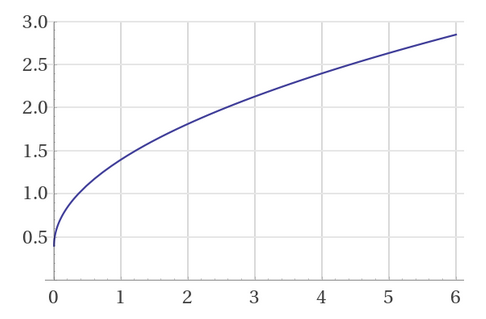
\includegraphics[width=3.0in]{graph_HW04_2.png}
%\vspace{-2mm}
%\caption{The position of a object (in meters) as a function of time
%  (in seconds). }
%\label{fig:graph2}
%\vspace{-5mm}
%\end{center}
%\end{figure}
  
  
\end{enumerate}

\end{document}




  \item Determine an equation for the linear function that generates
    the values in the table below.  

\begin{center}
\begin{tabular}{|| l | l ||}
\hline $x$ & $f(x)$ \\
\hline
5.2 & 27.8 \\
5.3 & 29.2 \\
5.4 & 30.6 \\
5.5 & 32.0 \\
5.6 & 33.4 \\
\hline
\end{tabular}
\end{center}





\end{document}
